\documentclass[aspectratio=169]{beamer}
\usepackage[utf8]{inputenc}
\usepackage[brazil]{babel}
\usepackage{multimedia,amsmath,graphicx,color,multicol,fancyhdr,amssymb,amsfonts,amsthm,setspace}
\usepackage{ragged2e}
\usetheme{Berlin}
\usecolortheme{dolphin}
\usepackage{setspace}
\usepackage{xcolor}
\usepackage{graphicx}


% Informações que serão inseridas no slide da capa:
\title[CETi Gilberto Mestrinho]{Revisão - PSC 1}
%\author[Prof. Joao Victor]{Prof. Joao Victor}
%\institute[IFAM]{Instituto Federal do Amazonas}
\date{\today} 
%\logo{
\includegraphics[scale=0.05]{logo-utfpr.png}} 

\newif\ifusarcorvermelha
%\usarcorvermelhatrue % Ativa o texto vermelho (comente para desativar)

% --- Comando \vermelho ---
\newcommand{\vermelho}[1]{%
    \ifusarcorvermelha
        {\color{red}#1}% % Texto vermelho se \ifusarcorvermelha = true
    \else
        #1% % Texto normal se \ifusarcorvermelha = false
    \fi
}

\begin{document}
\justifying
\onehalfspacing




\begin{frame}
    \begin{titlepage}
    \centering
    \vspace*{1cm} % Ajuste o espaçamento vertical conforme necessário
    
    % Logos alinhadas horizontalmente
    \noindent%
    \hspace*{0.3\paperwidth}%
    
\includegraphics[height=2cm,keepaspectratio]{logo_ufam.jpg}%
    \hfill%
    
\includegraphics[height=2cm,keepaspectratio]{logo_ceti.png}%
    \hspace*{0.3\paperwidth}%
    
    \vspace{0.1cm} % Espaço entre as logos e o título
    
    {\Large\textbf{Revisão - PSC 1}} \\ % Título do documento
    \vspace{1cm}
    {\large 5 de junho de 2025} % Data
    
    \vfill % Preenche o espaço vertical restante
    \end{titlepage}
\end{frame}

\section{Conteúdo Programático}

\begin{frame}{Conteúdo Programático - PSC I}

    \begin{center}
        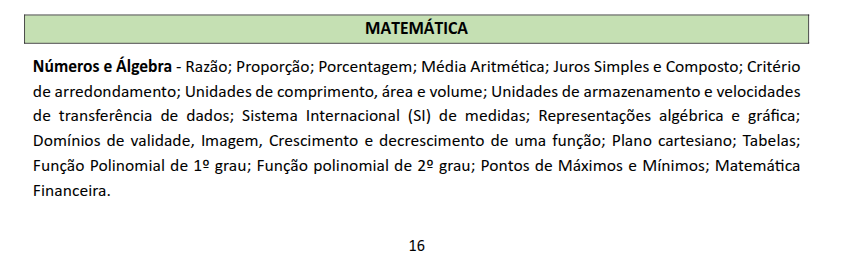
\includegraphics[scale=0.5]{p1.png}
    \end{center}
    
\end{frame}

\begin{frame}{Conteúdo Programático - PSC I}

    \begin{center}
        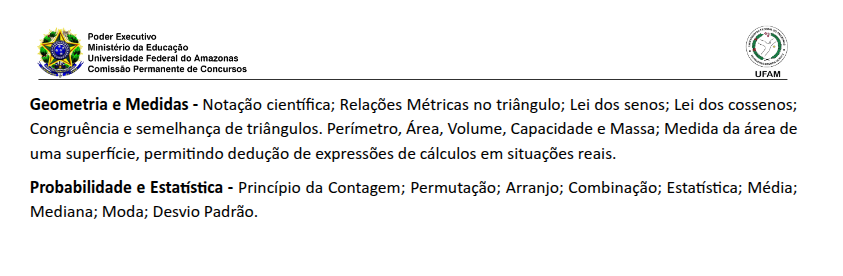
\includegraphics[scale=0.5]{p2.png}
    \end{center}
    
\end{frame}

\section{Questões PSC 1}

    \begin{frame}{PSC I - 2024 (Questão 47)}
        Suponha que, numa fábrica de calçados, o custo total da produção, em reais, é dado por $C(x) = x^{2}-40x+500$, em que $x$ é a quantidade de calçados produzidos. Nesse contexto, é \textbf{CORRETO} afirmar que:

            \begin{enumerate}[a]
                \item a produção de 100 calçados é a que realiza o custo máximo da produção.
                \item \vermelho{produção de 20 calçados é a que realiza o custo mínimo da produção}.  %
                \item quando são produzidos 40 calçados, o custo total da produção é de R\$ 1.600,00
                \item o custo máximo da produção é de R\$ 500,00
                \item o custo mínimo da produção é de R\$ 150,00
            \end{enumerate}
            
    \end{frame}


    \begin{frame}{PSC I - 2024 (Questão 49)}
        A área de um retângulo é $50 \ cm^{2}$ e sua base excede em 5 cm sua altura. A altura desse retângulo, nesse caso, mede:
        
            \begin{enumerate}[a]
                \item 6 cm.
                \item 4 cm.
                \item \vermelho{5 cm.} %
                \item 7 cm.
                \item 8 cm.
            \end{enumerate}
            
    \end{frame}

    \begin{frame}{PSC I - 2024 (Questão 50)}
    Um indivíduo aplicou R\$ 50.000,00 à taxa de $2\%$ a. m. - durante 6 meses - no regime de juros simples. Ao final dessa aplicação, o montante será de:

        \begin{enumerate}[a]
            \item $R\$ \ 60.000,00$
            \item $R\$ \ 52.000,00$
            \item $R\$ \ 54.000,00$
            \item $R\$ \ 58.000,00$
            \item \vermelho{$R\$ \ 56.000,00$} %
        \end{enumerate}
                
    \end{frame}


    \begin{frame}{PSC I - 2024 (Questão 51)}
        Num triângulo ABC, uma reta $r$ é paralela ao lado $\overline{BC}$ e divide o lado $\overline{AB}$ em dois segmentos de retas cujas medidas são 6 cm e 8 cm. Se o lado $\overline{AC}$ do triângulo mede 21 cm, então as medidas dos segmentos de reta formados pela intersecção da reta $r$ com o lado $\overline{AC}$ são:

        
        \begin{enumerate}[a]
            \item 8 cm e 13 cm.
            \item 6 cm e 15 cm.
            \item 7 cm e 14 cm.
            \item \vermelho{9 cm e 12 cm.} %
            \item 10 cm e 11 cm.
        \end{enumerate}
      
    \end{frame}


    \begin{frame}{PSC 2024 - (Questão 52)}
        Uma turma de trabalhadores construiu ${3}/{5}$ de uma obra em 15 dias. A partir desse momento, 6 trabalhadores deixaram a obra, que terminou com 4 dias de atraso. A quantidade de trabalhadores no início da obra era de:

            \begin{enumerate}[a]
                \item 40.
                \item 28.
                \item 30.
                \item 32.
                \item \vermelho{21.} %
            \end{enumerate}
    
    \end{frame}


    \begin{frame}{PSC I - 2024 (Questão 54)}
        A quadro a seguir apresenta quatro medições de uma determinada peça. 

        \begin{center}
            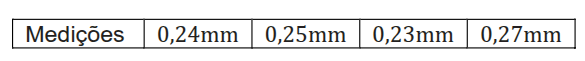
\includegraphics[scale=0.5]{psc2024Q54.png}
        \end{center} A média dessas medições é, aproximadamente,
        
            \begin{enumerate}[a]
                \item 0,27mm.
                \item 0,22mm.
                \item 0,23mm.
                \item \vermelho{0,25mm.} %
                \item 0,28mm.
            \end{enumerate}
    
    \end{frame}

    \begin{frame}{PSC I - 2023 (Questão 47)}
        Considere o gráfico ao lado. A lei que melhor representa a função afim $y=f(x)$ do gráfico é dada por:

        \begin{columns}
            \begin{column}{0.75\textwidth}
                \begin{enumerate}[a]
                    \item $f(x)=12-4x$
                    \item $f(x)=12-2x$
                    \item $f(x)=12+6x$
                    \item $f(x)=12+12x$
                    \item \vermelho{$f(x)=12-6x$}
                \end{enumerate}
            \end{column}

            \begin{column}{0.2\textwidth}
                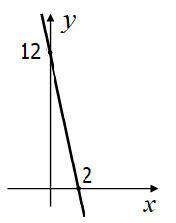
\includegraphics[width=\linewidth]{psc2023Q47.png}
            \end{column}
        \end{columns}
    
    \end{frame}

    \begin{frame}{PSC 2023 - (Questão 48)}
        Os triângulos ABC e PQR são congruentes. O perímetro do triângulo PQR é igual a 77 cm. Os lados do triângulo ABC medem, respectivamente, $x+7$, $3x+6$ e $4x$. Logo, o valor de $x$ é igual a:

            \begin{enumerate}[a]
                \item \vermelho{8} %
                \item 9
                \item 10
                \item 12
                \item 13
            \end{enumerate}
    
    \end{frame}

    \begin{frame}{PSC 2023 - (Questão 49)}
        Um estudante tem, em sua residência, internet com velocidade de $20\  MB/s$ . Ele precisa fazer o download de uma coletânea de exercícios, cujo arquivo zipado tem $1,5 \ GB$. Considerando que $1\ GB = 1024\ MB$, podemos afirmar que o intervalo de tempo necessário para que o arquivo zipado seja completamente baixado, caso a velocidade da internet se mantenha constante, será de:
        
            \begin{enumerate}[a]
                \item $65,0 \ s$
                \item $75,0 \ s$
                \item \vermelho{$76,8 \ s$} %
                \item $80,0 \ s$
                \item $90,8 \ s$
            \end{enumerate}
    
    \end{frame}

    \begin{frame}{PSC 2023 - (Questão 50)}
        Considere a função $f: \mathbb{R} \to \mathbb{R}$, definida por $f(x)=x^{2}-6x+4$. O menor valor que a função pode assumir é:

            \begin{enumerate}[a]
                \item $-6$
                \item $-7$
                \item $-3$
                \item $-4$
                \item \vermelho{$-5$} %
            \end{enumerate}
    
    \end{frame}

    \begin{frame}{PSC 2023 - (Questão 51)}
        Ana planeja fazer um empréstimo de $R\$ 45.000,00$ para reforma de sua loja de conveniência. Ela decidiu utilizar o sistema de amortização constante (SAC), calculado pela razão entre o capital contratado e a quantidade de parcelas. Ela pretende saldar a dívida em 4 anos. Nesse caso, o valor amortizado em cada parcela mensal será de:

            \begin{enumerate}[a]
                \item $R\$ \ 837,50.$
                \item $R\$ \ 737,50.$
                \item \vermelho{$R\$ \ 937,50.$} %
                \item $R\$ \ 1.152,50.$ 
                \item $R\$ \ 1.300,50.$ 
            \end{enumerate}
    
    \end{frame}

    \begin{frame}{PSC 2023 - (Questão 52)}
        A pontuação final para determinado Processo Seletivo é dada pela média ponderada dos pontos da prova de Conhecimentos Gerais, com peso 2, e dos pontos da prova de Conhecimentos Específicos, com peso 3. Considerando que determinado candidato obteve 175 pontos na prova de Conhecimentos Gerais e 155 pontos na prova de Conhecimentos Específicos, podemos afirmar que sua pontuação final foi de:

            \begin{enumerate}[a]
                \item \vermelho{163 pontos.} %
                \item 170 pontos.
                \item 280 pontos.
                \item 300,5 pontos.
                \item 407,5 pontos.
            \end{enumerate}
    
    \end{frame}

    \begin{frame}{PSC 2023 - (Questão 54)}
        A quantidade de números, com três algarismos distintos, que podemos formar com os algarismos 1, 2, 3, 4, 5, 6 e 8, é:

            \begin{enumerate}[a]
                \item 105.
                \item 330.
                \item 400.
                \item \vermelho{210.} %
                \item 540.
            \end{enumerate}
    
    \end{frame}
   
\end{document}
